\chapter{Motivation}

Social Engineering ist konträr zu seiner modernen Namensgebung sehrwohl bereits seit
Menschengedenken existent. Es lassen sich Beispiele von Social Engineering in der Mythologie,
Religion und Geschichte der Menschheit finden.
Unter den prominäntesten Beispielen ist das Trojanische Pferd\footnote{Es wird erzählt, dass
die Griechen den Krieg gegen Troja gewannen,
indem sich Odysseus die Social Engingeering Taktik ausdachte, das hölzerne Pferd zu bauen,
und die Trojaner zu manipulieren, dieses in die eigene Stadt zu bringen.}\bcite{origins}.

Social Engineering Angriffe nehmen im digitalen Zeitalter quantitativ kontinuierlich zu.
Sie zielen darauf ab durch Manipulation an sensible oder wertvolle Daten zu gelangen
und richten damit immensen Schaden an \bcite{seofwnep,4_mdpi}.
Diese Form von Angriffen richtet sich nicht nur gegen Unternehmen und Regierungsinstitutionen,
sondern auch gegen Individuen (insbesondere bezüglich Identitätsdiebstahl) \bcite{7_mdpi,verizon2012}.




\begin{figure}[H]
    \centering
    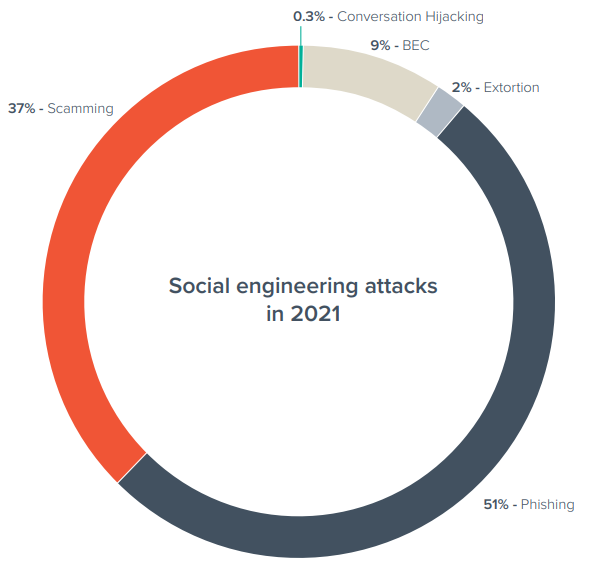
\includegraphics[scale=.5]{Barracuda_Social.Engineering.Attacks.png}
    \caption{Barracuda - Social Engineering Attacks}
\end{figure}

\begin{figure}[H]
    \centering
    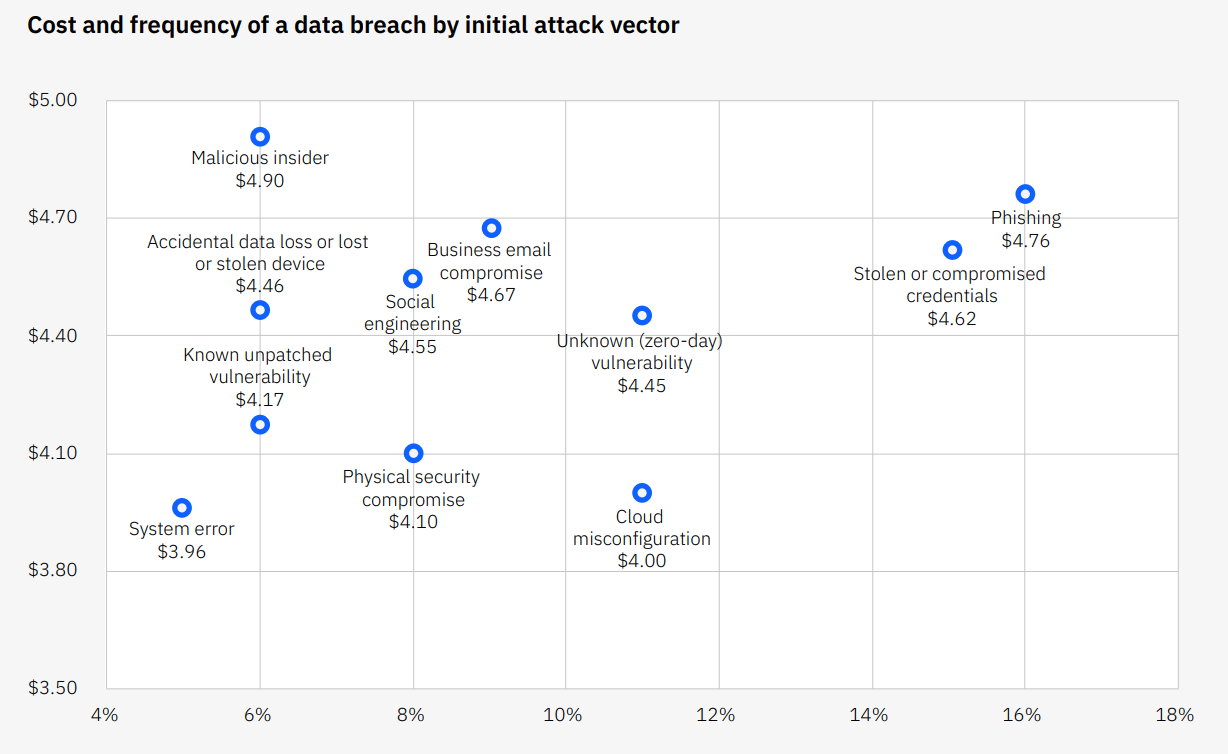
\includegraphics[width=5in]{IBM_Data.Breach.Report.png}
    \caption{IBM - Measured in USD millions}
\end{figure}
Avg. Kosten pro Breach (2022)

\newpage

"Actor Motives Financial (89\%), Espionage (11\%) (breaches)"\cite{verizon2022}
"Actor Motives Financial (95\%), Espionage (5\%) (breaches)"\cite{verizon2024}

conversation hijacking wenig ,denn verlangt etwas erfolg bei vorherigen angriffen.
z.b. folgt onversation hijacking oftmals auf account takeover.

"Hackers are starting to increasingly use phishing as part of their
ransomware attacks."\cite{3_barracuda}

"Extortion attacks make up only 2\% of the total number of
targeted phishing attacks we have seen in the past year. These
attacks were mostly sextortion email threats, where hackers
threaten to expose sensitive or embarrassing content to their
victim’s contacts unless a ransom is paid. Demands are usually
a few hundred or a few thousand dollars and need to be paid
in bitcoin, which is difficult to trace. In the UK, the number of
sextortion cases reported to National Crime Agency increased
by 88\% between 2018 and 2020, and the number is expected to
continue to increase"\cite{3_barracuda} stand 2021
stand 2024: Extortion: ($\sim$ 25\%) \cite{verizon2024}
Darunter fällt auch Ransomware

Pretexting: 2022 (27\%), 2024 (more than 40\%)
Phishing: 2022 ($\sim$ 70\%), 2024 (31\%)\cite{verizon2024,verizon2022}

"Account takeover is a form of identity theft and fraud where a
malicious third party successfully gains access to a user’s account
credentials"\cite{3_barracuda}
"Account takeover is one of the fastest growing threats. In 2021,
roughly 1 in 5 organizations (20\%) had at least one of their
Microsoft 365 accounts compromised. This means that in 2021
hackers managed to compromise around 500,000 Microsoft 365
accounts around the globe."\cite{3_barracuda}

Social Engineering MTTI (Mean Time To Identify): 218 Days
Social Engineering MTTC (Mean Time To Contain) :  80 Days\cite{6_ibmsecurity}


\section{Beispiele}

verweis auf film etc \dots
und trojanisches pferd, etc \dots
